	\chapter{Das Strahlungstransportproblem}
	\label{sec:radiative_transfer}
	
	Das Verhalten von Licht lässt sich (nach heutigem wissenschaftlichen Stand) durch die {\em Quantenelektrodynamik}\footnote{s. z.B. \citet{Feynman:1990p11684}} in allen Details vollständig beschreiben. Es beinhaltet Phänomene wie Dispersion, Brechung, Interferenz, Photon--Photon--Interaktion etc. Diese Effekte sind häufig dann am bedeutendsten, wenn die Ausmaße der betrachteten Objekte von der Größenordnung der Wellenlänge des Lichtes sind. Im Gegensatz dazu beschreibt die {\em geometrische Optik} die rein makroskopische lineare Ausbreitung großer Mengen von Photonen ohne Wellen--Phänomene zu berücksichtigen.
	
	Beim Strahlungstransportproblem (STP) sind wir an einer {\em phänomenologischen} Beschreibung interessiert. Das heißt wir wollen die Intensität des Lichts modellieren, die in typischen Anwendungen durch optische Instrumente (Auge, Teleskope mit Photoplatten/CCD--Chips) gemessen werden kann. Dies bedeutet, dass wir hauptsächlich eine geometrische Beschreibung des Lichts in Form eines Teilchentransportproblems ansetzen aber quantenmechanische Effekte wie Photonen--Streuung in erster Ordnung lokal mitberücksichtigen (z.B. in Form einer Streuphasenfunktion).
	
	Die folgende Darstellung und Herleitung orientiert sich an \citep{Arvo:1993p9035}.
	
	\section{Das Strahlungstransportproblem als Teilchentransportproblem}
	Um Strahlungstransport als Teilchentransportproblem behandeln zu können, müssen folgende Bedingungen erfüllt sein:
	\begin{itemize}
		\item{Die Teilchen müssen so klein und zahlreich sein, dass ihre statistische Verteilung als kontinuierlich angesehen werden kann}
		\item{Zu jedem Zeitpunkt lässt sich ein Teilchen komplett durch Position, Impuls und eventuelle interne Zustände (wie Polarisation, Frequenz, Ladung, Spin, etc.) charakterisieren}
	\end{itemize}
	Diese Annahmen sind für Photonen und die uns interessierenden räumlichen Entfernungen erfüllt.
	Darüber hinausgehend machen wir im Rahmen dieser Arbeit folgende Annahmen:
	\begin{itemize}
		\item{Die Materialeigenschaften ändern sich bei Variation des Ortes in der Größenordnung der Wellenlänge nur wenig}
		\item{Das Strahlungsintensitätsfeld ist stationär, d.h. innerhalb der typischen Zeiten, die ein Photon braucht um das Simulationsgebiet zu durchqueren, können die Materialeigenschaften als statisch angenommen werden}
		\item{Photonen werden ausschließlich elastisch gestreut}
		\item{der Raum wird als euklidisch angenommen, d.h. es werden keine relativistischen Effekte berücksichtigt}
	\end{itemize}
	Die Annahme ausschließlich elastischer Streuvorgänge erlaubt es uns, das Strahlungstransportproblem für jede Wellenlänge getrennt zu betrachten, da die Photonen ihre Wellenlänge nicht ändern und somit den Strahlungstransport in anderen Wellenlängen nicht beeinflussen. Daher behandeln wir im Folgenden nur eine Wellenlänge, da der polychromatische Fall immer als eine Reihe von monochromatischen Problemen behandelt werden kann. Aufgrund der monochromatischen (und damit monoenergetischen) Annahme ist der Impuls konstant. Daher genügt es zur vollständigen Beschreibung die Position $\location{r}$ (entsprechend drei Freiheitsgraden) und Bewegungsrichtung $\omega$ (entsprechend zwei Freiheitsgraden) eines Teilchens anzugeben. Wir können also jedes Teilchen mit einem Punkt im zugehörigen fünf--dimensionalen Phasenraum $\mathbb{R}^3 \times \mathcal{S}^2$ identifizieren, wobei $\mathbb{R}^3$ den euklidischen Raum und $\mathcal{S}^2=\{\location{x}\in\mathbb{R}^3| \|\location{x}\|=1\}$ die Einheitskugel im $\mathbb{R}^3$ bezeichnet.
	
	Um die statistische Verteilung unserer Teilchen im Phasenraum zu jedem Zeitpunkt spezifizieren zu können führen wir die Phasenraumdichte $n$ ein, sodass $$n(\location{r},\omega,t)\,d\location{r}\,d\omega$$ der Anzahl Teilchen entspricht, die sich zum Zeitpunkt $t$ in einem infinitesimalen Volumen $d\location{r}$ um $\location{r} \in \mathbb{R}^3$ befinden und sich in eine Richtung bewegen, die innerhalb eines infinitesimalen Raumwinkels $d\omega$ um $\omega \in \mathcal{S}^2$ liegt. Damit hat $n$ die Einheit $\text{m}^{-3}\text{sr}^{-1}$. Die Phasenraumdichte trifft keine Aussage über Materialeigenschaften oder innere Zustände der Teilchen, wie Masse oder Frequenz, sondern beschreibt lediglich deren Anzahldichte im Phasenraum. Physikalische Observablen (wie z.B. die Intensität) führen wir später (in Abschnitt \ref{subsec:strahlungsgroessen}) auf diese Phasenraumdichte zurück. An dieser Stelle erlaubt die abstrakte Natur von $n$ eine klare Darstellung des Photonentransports. Aus der Phasenraumdichte lassen sich alle für uns interessanten Größen ableiten, für die folgende Herleitung ist es aber besser die Rate zu betrachten, mit der Teilchen eine imaginäre Fläche durchqueren.
	
	Sei $dA$ ein infinitesimales Flächenelement, $\omega$ seine Flächennormale und $d\omega$ ein infinitesimales Raumwinkelelement, das $\omega$ beinhaltet (s. Abb.~(\ref{fig:phasespacefluxsurface})). Betrachten wir nun die Teilchen, welche die Fläche $dA$ in einem Zeitraum $dt$ mit Bewegungsrichtung innerhalb $d\omega$ passieren. Alle diese Teilchen liegen im Volumen $dV=dA\,ds$ wobei $ds=v\,dt$ und $v$ die Geschwindigkeit der Teilchen ist. Wenn $\location{r}$ innerhalb des Volumens $dV$ liegt, ist die Anzahl der Teilchen $$n(\location{r},\omega,t)\,\underbrace{dA\,ds}_\text{dV}\,d\omega.$$ Wenn wir stattdessen aber nach der Rate fragen, mit der die Teilchen $dA$ passieren, erhalten wir den Phasenraumfluss $$\phi(\location{r},\omega,t):=v\,n(\location{r},\omega,t)$$ mit der Einheit $[\phi]=\text{m}^{-2}\text{sr}^{-1}s^{-1}$. Die Teilchenanzahl in $dV$ mit dem Phasenraumfluss ausgedrückt ist $$dN=\phi(\location{r},\omega,t)\,dA\,d\omega\,dt.$$
	\begin{figure}
		\centering
		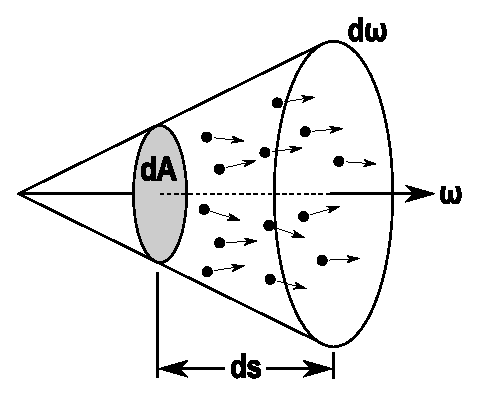
\includegraphics[height=0.3\textheight]{phasespacefluxsurface.eps}
		\caption{Teilchen, die das infinitesimale Flächenelement $dA$ durchqueren und sich in eine Richtung innerhalb des infinitesimalen Raumwinkelelements $d\omega$ um die Flächennormale $\omega$ von $dA$ bewegen.}
		\label{fig:phasespacefluxsurface}
	\end{figure}
	Der Phasenraumfluss ist wie die Phasenraumdichte eine fundamentale Größe, aus der wir alle anderen Observablen ableiten können. Im Folgenden werden wir uns meist auf den Phasenraumfluss beziehen.
		
	Unser Ziel ist es nun eine Bilanzgleichung für Teilchen in einem beliebigen Teil $V \times \Omega$ des Phasenraums (s. Abb.~(\ref{fig:phasespacevolume})) aufzustellen. Dafür sei $V \subset \mathbb{R}^3$ ein Teilvolumen des $\mathbb{R}^3$ und $\Omega \subset \mathcal{S}^2$ ein beliebiger Raumwinkel aus der Einheitskugel $\mathcal{S}^2$. Dazu untersuchen wir Ursachen für eine Veränderung der Teilchenzahl in unserem betrachteten Phasenraumvolumen $V \times \Omega$.
	\begin{figure}
		\centering
		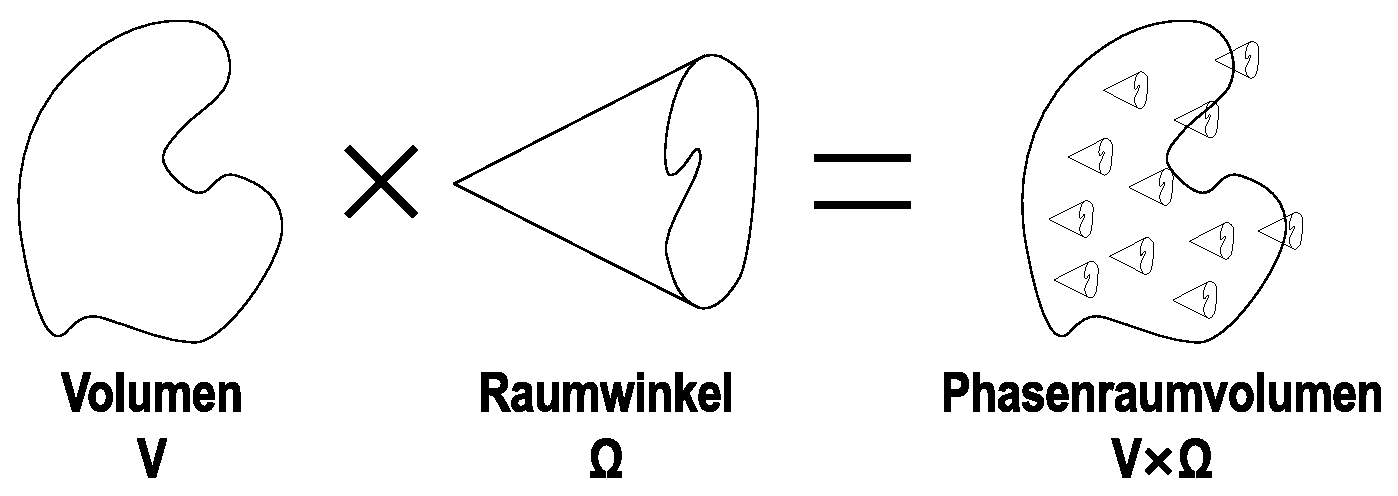
\includegraphics[width=0.8\textwidth]{phasespacevolume.eps}
		\caption{Darstellung einer Teilmenge $V \times \Omega$ des Phasenraums. Sie repräsentiert alle Teilchen, die sich innerhalb des Volumens $V$ befinden und sich in eine Richtung $\omega\in\Omega$ bewegen.}
		\label{fig:phasespacevolume}
	\end{figure}

	Zur {\em Emission} zählt jeder Prozess, der neue Teilchen erzeugt, wie z.B. chemische Reaktionen, thermische Emission oder Kernfusion. Emission innerhalb von $V$ in eine Richtung $\omega\in\Omega$ stellt also eine Quelle für Teilchen dar. Nach der Emission bewegen sich die Teilchen in unserem Modell gradlinig mit konstanter Geschwindigkeit bis eine Wechselwirkung mit dem Medium stattfindet. Bewegt sich ein Teilchen bei seiner gradlinigen Bewegung in das Volumen $V$ hinein oder aus ihm heraus und bewegt es sich dabei in eine Richtung innerhalb von $\Omega$, so ändert dies ebenfalls die Bilanz. In diesem Fall sprechen wir von {\em Durchströmen}. Findet eine {\em Kollision} des Teilchens mit dem Medium statt, kann das Teilchen entweder absorbiert oder gestreut werden. Wird es absorbiert wirkt dies als Teilchensenke. Wird es gestreut, dann kann es, je nach Richtung vor und nach der Kollision, entweder keinen Einfluss auf die Teilchenbilanz haben (Bewegungsrichtung vor und nach der Kollision entweder innerhalb oder außerhalb von $\Omega$), es kann herausgestreut werden (Bewegungsrichtung vor der Kollision innerhalb und nach der Kollision ausserhalb von $\Omega$) oder aber hineingestreut werden (Bewegungsrichtung vor der Kollision ausserhalb und nach der Kollision innerhalb von $\Omega$) werden.
	
	Um die einzelnen Beiträge dieser Prozesse zur Teilchenbilanz quantitativ zu erfassen führen wir die Teilchenzahl $$N(t):=\int_\Omega \int_V n(\location{r},\omega,t)\,d\location{r}\,d\omega$$ ein. Sie gibt an wieviele Teilchen sich zum Zeitpunkt $t$ im Phasenraumvolumen $V \times \Omega$ befinden. Durch die eben beschriebenen Prozesse ändert sich $N(t)$ normalerweise mit der Zeit. Ist die Zeit, die ein Teilchen benötigt um das System zu durchqueren, klein gegenüber der typischen Zeitskala für Veränderung des Systems, können wir annehmen, dass sich die Teilchenzahl überall im dynamischen Gleichgewicht befindet, d.h. dass Teilchen ständig aus dem Phasenraumvolumen hinein- und hinausströmen, erzeugt, absorbiert und gestreut werden, aber sich alle Prozesse die Waage halten, $N(t)$ also stationär ist:$$\frac{dN}{dt}=0\qquad\left[\frac{1}{\text{s}}\right].$$ Teilen wir diese Änderung von $N$ mit der Zeit auf die erläuterten Prozesse auf, sind wir bei der Bilanzgleichung angelangt:$$\frac{dN}{dt}=\begin{bmatrix}\text{Änderung}\\ \text{durch}\\ \text{Emission}\end{bmatrix}+\begin{bmatrix}\text{Änderung}\\ \text{durch}\\ \text{Durchströmung}\end{bmatrix}+\begin{bmatrix}\text{Änderung}\\ \text{durch}\\ \text{Kollisionen}\end{bmatrix}=0.$$ Wir leiten nun für jeden dieser Ausdrücke einen Formelausdruck her.
	Die Änderung aufgrund von Emission nennen wir $$\mathbf{E}=\int_\Omega \int_V q(\location{r},\omega)\,d\location{r}\,d\omega\qquad\left[\frac{1}{\text{s}}\right],$$ wobei wir die Quellfunktion $q$ (mit Einheit $\text{m}^{-3}\text{sr}^{-1}\text{s}^{-1}$) eingeführt haben, die für jeden Ort $\location{r}$ und jede Raumrichtung $\omega$ die Anzahl pro Sekunde, Einheitsvolumen und Einheitsraumwinkel erzeugter Teilchen angibt. Hinein- und herausströmende Teilchen erzeugen eine Teilchenrate
	$$\mathbf{S}=\int_\Omega \int_{\partial V} \phi(\location{r},\omega)(\omega \cdot \location{n}(\location{r}))d\location{r}\,d\omega,$$
	die wir durch Integrieren über $\partial V$ (die Oberfläche von V) erhalten. Hierbei steht $\location{n}(\location{r})$ für die Flächennormale am Ort $\location{r}\in\partial V$. Das Skalarprodukt zwischen Bewegungsrichtung $\omega$ und Flächennormalen sorgt für das richtige Vorzeichen, wobei ein positiver Wert Teilchenverlust bedeutet.
	Der letzte Beitrag $\mathbf{C}$ trägt den Kollisionen Rechnung. Da Teilchen nur mit dem Medium, nicht aber untereinander interagieren, muss die Kollisionsrate unabhängig von $\phi$ sein. Wir unterteilen $\mathbf{C}$ in einen Absorptionsteil und einen Streuanteil:
	$$\mathbf{C}=\mathbf{C}_\text{abs}+\mathbf{C}_\text{sca}.$$
	Wir nehmen an, dass die Wahrscheinlichkeit einer Absorption proportional zur zurückgelegten Distanz im Medium ist und unabhängig von der Bewegungsrichtung, was gleichbedeutend mit der Annahme eines isotropen Mediums ist. Die Proportionalitätskonstante am Ort $\location{r}$ nennen wir den (Volumen-)Absorptionsquerschnitt $\kappa(\location{r})$ ($[\kappa]=\frac{1}{\text{m}}=\frac{m^2}{m^3}$). Die zugehörige Teilchenrate ist
	$$\mathbf{C}_\text{abs}=\int_\Omega \int_V \kappa(\location{r})\phi(\location{r},\omega)\,d\location{r}\,d\omega.$$
	Die genauen Mechanismen der Streuung werden bei der Lösung der Wellengleichung behandelt (Mie--Theorie). In unserem Teilchentransport repräsentieren wir diese Streumodelle durch die Streuphasenfunktion $k(\location{r},\omega,\omega')$ und den Volumenstreuquerschnitt $\sigma(\location{r})$. Dabei gibt $k(\location{r},\omega,\omega')$ bei Streuung eines aus Richtung $\omega$ kommenden Teilchens am Ort $\location{r}$ die Wahrscheinlichkeit pro Einheitsraumwinkel an, nach $\omega'$ gestreut zu werden. Da ein gestreutes Teilchen erhalten bleibt, gilt für $k$ die Normierungsbedingung
	\begin{equation}\label{eq:k_norm_req}
	  \int_{\mathcal{S}^2} k(\location{r},\omega,\omega')\,d\omega'=1.
	\end{equation}
	Außerdem ist $k$ symmetrisch bezüglich Vertauschung der Bewegungsrichtungen vor und nach der Streuung:
	$$k(\location{r},\omega,\omega')=k(\location{r},\omega',\omega)\quad \forall\:\omega,\omega'\in\mathcal{S}^2.$$
	Beide Bedingungen werden z.B. durch die isotrope Streuphasenfunktion $$k_\text{iso}(\location{r},\omega,\omega')=\frac{1}{4\pi}$$ erfüllt.
	Wie bei der Absorption, nehmen wir an, dass die Wahrscheinlichkeit eines Teilchens gestreut zu werden von der durch das Medium zurückgelegten Distanz, nicht aber von der Bewegungsrichtung abhängt. Wir teilen $\mathbf{C}_\text{sca}$ weiter auf, in einen Teil
	$$\mathbf{C}_\text{out}=\int_\Omega \int_V \int_{\mathcal{S}^2} \sigma{(\location{r})}k(\location{r},\omega,\omega')\phi(\location{r},\omega)\,d\omega'\,d\location{r}\,d\omega,$$
	der herausgestreute Teilchen berücksichtigt, sowie einen Teil
	$$\mathbf{C}_\text{in}=\int_\Omega \int_V \int_{\mathcal{S}^2} \sigma{(\location{r})}k(\location{r},\omega',\omega)\phi(\location{r},\omega')\,d\omega'\,d\location{r}\,d\omega$$
	entsprechend für hineingestreute Teilchen. Dabei sollte erwähnt werden, dass sowohl $\mathbf{C}_\text{out}$ als auch $\mathbf{C}_\text{in}$ Teilchen berücksichtigen, deren Richtung vor und nach der Streuung in $\Omega$ liegt, was weder einem Zuwachs noch einem Verlust an Teilchen entspricht. Da für unsere Bilanz aber immer nur die Differenz von $\mathbf{C}_\text{out}$ und $\mathbf{C}_\text{in}$ betrachtet wird, hebt sich dieser Teil wieder heraus. Alternativ könnten wir auch über $\mathcal{S}^2 \setminus \Omega$ integrieren, was zu einer komplizierteren Rechnung, aber zu keinem anderen Endergebnis führen würde. Fügen wir die Einzelterme zusammen und ordnen nach Zuwächsen und Verlusten sieht unsere Bilanzgleichung für die Teilchenraten in $V \times \Omega$ wie folgt aus:
	$$\underbrace{\mathbf{S}+\mathbf{C}_\text{abs}+\mathbf{C}_\text{out}}_\text{Verluste}=\underbrace{\mathbf{E}+\mathbf{C}_\text{in}}_\text{Zuwächse}$$
	Es fällt bei der Betrachtung der Formeln für die einzelnen Terme auf, dass alle Terme bis auf $\mathbf{S}$ Volumenintegrale über $V$ enthalten. $\mathbf{S}$ enthält stattdessen ein Oberflächenintegral über $\partial V$. Mit dem Gauss'schen Satz erhalten wir
	$$\mathbf{S}=\int_\Omega \int_V \omega \cdot (\nabla\phi)(\location{r},\omega)\,d\location{r}\,d\omega,$$
	wobei wir $$\nabla \cdot(\omega\phi)=\omega\cdot(\nabla\phi)+\underbrace{(\nabla\omega)}_{=0}\cdot\,\phi$$ benutzt haben.
	
	In der Bilanzgleichung treten jetzt nur noch Volumenintegrale über $V \times \Omega$ auf. Da $V$ und $\Omega$ beliebig gewählt waren, erhalten wir den lokalen Zusammenhang:
	\begin{multline*}
	  \omega\cdot\nabla\phi(\location{r},\omega)+\kappa(\location{r})\phi(\location{r},\omega)+\int_{\mathcal{S}^2}\sigma(\location{r})k(\location{r},\omega,\omega')\phi(\location{r},\omega)d\omega' \\
	  =q(\location{r},\omega)+\int_{\mathcal{S}^2}\sigma(\location{r})k(\location{r},\omega',\omega)\phi(\location{r},\omega')d\omega'.
	\end{multline*}
	Da beim $\mathbf{C}_\text{out}$--Integral $\sigma$ und $\phi$ nicht von der Integrationsvariable abhängen und sich das verbleibende Integral aufgrund der Normierung (\ref{eq:k_norm_req}) vereinfacht, ergibt sich schließlich die Bilanzgleichung in Gestalt einer Integro--Differentialgleichung in $\phi$:
	\begin{equation}\label{eq:particle_balance_equation}
	  \omega\cdot\nabla\phi(\location{r},\omega)+\left(\kappa(\location{r})+\sigma(\location{r})\right)\phi(\location{r},\omega)
	  =q(\location{r},\omega)+\sigma(\location{r})\int_{\mathcal{S}^2}k(\location{r},\omega',\omega)\phi(\location{r},\omega')d\omega'
	\end{equation}
	Im folgenden Abschnitt stellen wir den Bezug zwischen unseren abstrakten Teilchentransportgrößen und physikalischen Strahlungsgrößen her.

	\section{Phänomenologische Strahlungsgrößen}\label{subsec:strahlungsgroessen}
	Im vorigen Abschnitt haben wir das Strahlungstransportproblem bewusst auf ein Teilchentransportproblem (mit abstrakten Teilchen statt Photonen) reduziert um einerseits eine klare Herleitung zu ermöglichen und um andererseits die Verwandtschaft zu anderen Transportproblemen (wie z.B. Neutronentransport) offensichtlich zu machen. Für den Anschluss zu radiometrischen Strahlungsgrößen, ersetzen wir die abstrakten Teilchen durch Photonen. Photonen haben zwei Eigenschaften die wir berücksichtigen müssen. Sie bewegen sich konstant mit Lichtgeschwindigkeit, d.h. wir können die vorher gebrauchte allgemeine Teilchengeschwindigkeit $v$ gleich $\text{c}$ setzen. Außerdem besitzt jedes Photon eine Energie, die mit seiner Frequenz $\nu$ über 
	$$E=h\nu \qquad[J]$$
	zusammenhängt. Dabei bezeichnet $h$ das Planck'sche Wirkungsquantum.
	Jeder Frequenz $\nu$ können wir ein monochromatisches Transportproblem zuordnen, dessen Lösung in Form eines Phasenraumflusses $\phi_\nu$ die Photonenfrequenz als Index trägt.
	Die {\em spezifische Intensität} $I_\nu(\location{r},\omega)$ erhalten wir nun aus dem Phasenraumfluss bzw. der Phasenraumdichte gemäß
	\begin{align}\label{eq:intensity_def}
		I_\nu(\location{r},\omega)d\nu & = h\nu\,\phi_\nu(\location{r},\omega)\\
		                       & = c h\nu\,n_\nu(\location{r},\omega) \qquad \left[\frac{\text{W}}{\text{m}^2\text{sr}}\right] \nonumber
	\end{align}
	Sie gibt an, wieviel Joule am Ort $\location{r}$ pro Sekunde durch eine Einheitsfläche mit Flächennormale $\omega$ pro Einheitsraumwinkel in Richtung $\omega$ und pro Frequenzintervall durch Photonen mit Frequenz $\nu$ transportiert wird:
	$$dE_\nu=I_\nu(\location{r},\omega) dA\,dt\,d\omega\,d\nu.$$
	Wir führen außerdem die {\em spezifische Emissivität} $\varepsilon_\nu$ ein. Wir erhalten Sie aus der Quellfunktion $q_\nu$ durch
	\begin{equation}\label{eq:emissivity_def}
		\varepsilon_\nu(\location{r},\omega)d\nu = h\nu\,q_\nu(\location{r},\omega) \qquad \left[\frac{\text{W}}{\text{m}^3\text{sr}}\right].
	\end{equation}
	
	Multiplizieren wir die abstrakte Transportgleichung (\ref{eq:particle_balance_equation}) mit $h\nu$ und benutzen wir die Beziehungen (\ref{eq:intensity_def}, \ref{eq:emissivity_def}) erhalten wir mit
	\begin{equation}\label{eq:stg_diff}
	  \omega\cdot\nabla I_\nu(\location{r},\omega)+\left(\kappa_\nu(\location{r})+\sigma_\nu(\location{r})\right)I_\nu(\location{r},\omega)
	  =\varepsilon_\nu(\location{r},\omega)+\sigma_\nu(\location{r})\int_{\mathcal{S}^2}k_\nu(\location{r},\omega',\omega)I_\nu(\location{r},\omega')d\omega'
	\end{equation}
	die {\em Strahlungstransportgleichung in differentieller Form}. Sie stellt eine In\-te\-gro--Dif\-fe\-ren\-ti\-al\-glei\-chung für $I_\nu$ auf dem 5--dimensionalen Phasenraum $\mathbb{R}^3 \times \mathcal{S}^2$ dar und kann für jede Frequenz $\nu$ getrennt gelöst werden. Sie gibt für jede Kombination aus Ort $\location{r}$ und Ausbreitungsrichtung $\omega$ das lokal zu erfüllende Gleichgewicht aus Verlusten (linke Seite) und Zuwächsen (rechte Seite) an.
	
	Wir fassen die Verluste durch Absorption und Streuung mit dem {\em Vo\-lu\-men\-ex\-tink\-ti\-ons\-quer\-schnitt}
	$$\xi_\nu(\location{r}):=\kappa_\nu(\location{r})+\sigma_\nu(\location{r}) \qquad\left[\frac{1}{m}\right]$$
	zusammen, wodurch wir (\ref{eq:stg_diff}) auch kürzer als
	\begin{equation}\label{eq:stg_diff2}
	  \omega\cdot\nabla I_\nu(\location{r},\omega)+\xi_\nu(\location{r})I_\nu(\location{r},\omega)
	  =\varepsilon_\nu(\location{r},\omega)+\sigma_\nu(\location{r})\int_{\mathcal{S}^2}k_\nu(\location{r},\omega',\omega)I_\nu(\location{r},\omega')d\omega'
	\end{equation}
	schreiben können.
	Außerdem definieren wir die dimensionslose {\em optische Tiefe}
	\begin{equation*}
		\tau_\nu(\location{r}_1,\location{r}_2):=\int_{s=0}^{\|\location{r}_2-\location{r}_1\|} \xi_\nu(\location{r}_1+s(\location{r}_2 - \location{r}_1))\,ds,
	\end{equation*}
	als Maß für die Undurchsichtigkeit des Mediums bei der Frequenz $\nu$ zwischen zwei Orten $\location{r}_1$ und $\location{r}_2$. Vereinfachen wir Gleichung (\ref{eq:stg_diff2}), indem wir Quellen zu Null setzen und eine beliebige Richtung $\omega$ wählen, so gelangen wir zur gewöhnlichen Differentialgleichung
	$$I_\nu'(s)+\xi_\nu(s)I_\nu(s)=0,$$
	die durch
	\begin{equation}
		I_\nu(s)=I_\nu(0)\:\text{exp}\left(-\int_{s'=0}^s \xi_\nu(s')\right)=I_\nu(0)\:\text{exp}\left(-\tau_\nu(0,s)\right)
		\label{eq:exponentialdecay}
	\end{equation}
	gelöst wird. Die optische Tiefe beschreibt also eine exponentielle Abschwächung einfallender Intensität. Nach der Definition der verschiedenen phänomenologischen Strahlungsgrößen schauen wir uns nun an, wie ihre Messung aufgefasst und mathematisch definiert werden kann.
	
	
	\section{Die Messgleichung}\label{sec:measurement_equation}
	Mit dem Strahlungsintensitätsfeld, das aus der Gesamtheit aller spezifischen Intensitäten $I_\nu$ besteht, meinen wir die Funktion
	$$I:\mathbb{R}_+\times\mathbb{R}^3\times\mathcal{S}^2\to\mathbb{R}_+\;,\qquad (\nu,\location{r},\omega)\mapsto I_\nu(\location{r},\omega),$$
	die vom 6--dimensionalen Raum aller Frequenzen, Orte und Raumrichtungen auf die lokale spezifische Intensität abbildet.
	
	Funktionen dieser Art bilden einen Skalarproduktraum. Das Null--Element ist die konstant auf Null abbildende Funktion. Zwei Funktionen lassen sich punktweise addieren und ergeben so eine neue Funktion, die auch nach $\mathbb{R}_{\geq 0}$ abbildet. Das Skalarprodukt zwischen zwei Funktionen $f$ und $g$ ist schließlich mit
	$$\langle f,g\rangle=\int_{\mathbb{R}_+} \int_{\mathbb{R}^3} \int_{\mathcal{S}^2} f(\nu,\location{r},\omega)g(\nu,\location{r},\omega)\,d\omega\,d\location{r}\,d\nu$$
	gegeben.
	
	Mit diesem funktionalanalytischen Handwerkszeug definieren wir eine Messung als das Skalarprodukt zwischen unserem Strahlungsintensitätsfeld $I$ und einer {\em Sensitivitätsfunktion} $W$, welche die Stärke der Gewichtung angibt, mit der die spezifische Intensität der Frequenz $\nu$ am Ort $\location{r}$ in Richtung $\omega$ in den Messwert eingeht. Die entsprechende Formel
	\begin{equation}\label{eq:messgleichung}
		M^{(i)}:=\langle W^{(i)},I\rangle=\int_{\mathbb{R}_+} \int_{\mathbb{R}^3} \int_{\mathcal{S}^2} W^{(i)}(\nu,\location{r},\omega)I_\nu(\location{r},\omega)\,d\omega\,d\location{r}\,d\nu
	\end{equation}
	nennen wir {\em Messgleichung} (für den $i$--ten Sensor). Für monochromatische Messungen führen wir zusätzlich noch 
	\begin{equation}\label{eq:messgleichung_mono}
		M_\nu^{(i)}:=\langle W_\nu^{(i)},I_\nu\rangle=\int_{\mathbb{R}^3} \int_{\mathcal{S}^2} W_\nu^{(i)}(\location{r},\omega)I_\nu(\location{r},\omega)\,d\omega\,d\location{r}
	\end{equation}
	ein, womit wir (\ref{eq:messgleichung}) auch als
	\begin{equation}\label{eq:messgleichung_frommonos}
		M^{(i)}=\int_{\mathbb{R}_+} M_\nu^{(i)}\,d\nu
	\end{equation}
	schreiben können.
	Diese Abstraktion erlaubt uns größtmögliche Freiheit beim kreieren virtueller Sensoren. Beispielsweise könnte $W$ nur in einem kleinen Volumen und einem kleinen Raumwinkel, aber bei allen Frequenzen, nichtverschwindend sein, und so einen Sensor zur Messung der Gesamt--Intensität an einem bestimmten Ort in eine bestimmte Richtung repräsentieren. Ebenso kann durch gleichstarke Gewichtung aller Raumrichtungen die mittlere Intensität gemessen werden.
	
	Was zunächst nur als theoretisches Konstrukt ohne praktischen Nutzen erscheint, wird sich später in Verbindung mit Monte--Carlo--Sampling als vielseitiges und effizientes Werkzeug erweisen.
	
	
	%\section{Übersicht etablierter Lösungsverfahren}
	%TODO: Übersicht benutzter Lösungsverfahren, Meilensteine (wann zum ersten mal Polarisation gerechnet?, Warum etablieren sich MC-Verfahren so spät?, etc...)
		
	\chapter{Pfadintegralformulierung der Strahlungstransportgleichung}\label{chapter:path_radiative_transfer}
	In diesem Abschnitt leiten wir eine alternative Formulierung der Strahlungstransportgleichung einerseits und ihrer Lösung (genauer von Messungen der Lösung im Sinne von (\ref{eq:messgleichung})) andererseits her. Dies führt uns zu einem besseren Verständnis des Strahlungstransports und gibt uns darüber hinaus neue Ansatzpunkte zur effizienten Lösung des Strahlungstransportproblems.
	
	Die Idee zu dieser Formulierung stammt aus der Dissertation von \citet{Veach:1997p9136}, wird aber schon in \citep{Arvo:1995p9257} vorgestellt. Beide Dissertationen behandeln allerdings nur den Strahlungstransport zwischen Oberflächen. In der Arbeit von \citet{Pauly:2000p5705} wird dies auf partizipierende Medien ausgedehnt. Aus \citep{Arvo:1993p9035} stammt außerdem die Herleitung der integralen Form der Strahlungstransportgleichung.
	
	
	\section{Strahlungstransportgleichung in integraler Form}
	Für diesen und die folgenden Abschnitte lassen wir den Index $\nu$ aus Übersichtsgründen weg, womit gemeint ist, dass wir stellvertretend für alle Frequenzen ein einzelnes monochromatisches Strahlungstransportproblem einer beliebigen Frequenz nehmen. Wenn wir zum polychromatischen Fall zurückkehren führen wir die Indizes wieder ein.
	
	In differentieller Form nimmt die Strahlungstransportgleichung, wie wir in Abschnitt (\ref{subsec:strahlungsgroessen}) gesehen haben dann folgende Gestalt an:
		\begin{equation}
			\omega \cdot \nabla I(\location{r},\omega)+\overbrace{\left(\kappa(\location{r})+\sigma(\location{r})\right)}^{=:\xi(\location{r})}I(\location{r},\omega)=\varepsilon(\location{r},\omega)+\sigma(\location{r}) \int_{\mathcal{S}^2} k(\location{r},\omega',\omega)I(\location{r},\omega') d\omega'.
			\label{eq:diff.STG}
		\end{equation}
	
	Schreiben wir das Skalarprodukt zwischen $\omega$ und dem $\nabla$--Operator als Richtungsableitung
	\newcommand{\dds}{\frac{\text{d}}{\text{d}s}}
	\newcommand{\ddszero}{\left. \dds \right|_{s=0}}
	\begin{equation*}
		\omega \cdot \nabla I(\location{r},\omega)
		=  \ddszero I(\location{r}+s\,\omega,\omega)
		=  -\ddszero I(\location{r}-s\,\omega,\omega)
	\end{equation*}
	können wir (\ref{eq:diff.STG}) als
	\begin{multline}
		\dds I(\location{r}-s\,\omega,\omega) - \xi(\location{r}-s\,\omega)I(\location{r}-s\,\omega,\omega) = \\-\varepsilon(\location{r}-s\,\omega,\omega) -\sigma(\location{r}-s\,\omega) \int_{\mathcal{S}^2} k(\location{r}-s\,\omega,\omega',\omega)I(\location{r}-s\,\omega,\omega') \text{d}\omega'
		\label{eq:diff.STGtranslated}
	\end{multline}
	umschreiben. Dabei haben wir die Beschränkung $s=0$ fallengelassen, was die Korrektheit der Umformung aber nicht ändert. Mit den Abkürzungen
	\begin{align*}
		{\hat I}(s)&:=I(\location{r}-s\,\omega,\omega) \\
		Q(\location{r},\omega)&:= \varepsilon(\location{r},\omega)+\sigma(\location{r}) \int_{\mathcal{S}^2} k(\location{r},\omega',\omega)I(\location{r},\omega') d\omega' \\
		{\hat Q}(s)&:=Q(\location{r}-s\,\omega,\omega)\\
		{\hat \xi}(s)&:=\xi(\location{r}-s\,\omega) \\
		{\hat \tau}(s)&:= \int_{s'=0}^{s} {\hat \xi}(s') \text{d}s'
	\end{align*}
	wird aus (\ref{eq:diff.STGtranslated})
	\begin{equation}
		\dds {\hat I}(s) - {\hat \xi}(s){\hat I}(s)= -{\hat Q}(s) \qquad |\cdot e^{-{\hat \tau}(s)}.
		\label{eq:diff.STGhatted}
	\end{equation}
	Gleichung (\ref{eq:diff.STGhatted}) ist eine gewöhnliche Differentialgleichung die sich mit
	\begin{align}
		(\ref{eq:diff.STGhatted})\Leftrightarrow\qquad \dds \left(e^{-{\hat \tau}(s)} {\hat I}(s)\right)&= -e^{-{\hat \tau}(s)} {\hat Q}(s) \qquad | \int_{s'=0}^s (\cdot)\text{d}s' \nonumber \\
		\Leftrightarrow\qquad e^{-{\hat \tau}(s)} {\hat I}(s) - {\hat I}(0) &= -\int_{s'=0}^s e^{-{\hat \tau}(s')} {\hat Q}(s') \text{d}s' \nonumber \\
		\Leftrightarrow\qquad {\hat I}(0) &= e^{-{\hat \tau}(s)} {\hat I}(s) + \int_{s'=0}^s e^{-{\hat \tau}(s')} {\hat Q}(s') \text{d}s' \label{eq:diff.STGpreintegral}
	\end{align}
	leicht nach ${\hat I}(0)$ auflösen lässt. Obwohl ${\hat Q}(s)$ lokal die Intensität $I$ über alle Raumrichtungen integriert, dürfen wir die Lösung von (\ref{eq:diff.STGhatted}) $Q$ als unabhängig von $I$ behandeln, da die Schnittmenge zwischen der Geraden im Raum, auf der wir die Differentialgleichung lösen, und der Menge aller Raumrichtungen $\mathcal{S}^2$ bei der Integration über alle Raumrichtungen eine Nullmenge ist und somit für physikalisch relevante Strahlungsintensitätsfelder (d.h. solche, die hinreichend stetig/beschränkt bzw. keine Delta--Distribution sind) keinen Beitrag zum Integral leistet.
	Setzen wir in (\ref{eq:diff.STGpreintegral}) die ursprünglichen Ausdrücke ein, erhalten wir die {\em Strahlungstransportgleichung in integraler Form}:
	\begin{multline}
		I(\location{r},\omega) = e^{-\tau(\location{r},\location{r}-s\,\omega)} {\hat I}(\location{r},\location{r}-s\,\omega) + \int_{s'=0}^\infty e^{-\tau(\location{r},\location{r}-s\,\omega)} \;\cdot \\
		\quad\cdot\left( \varepsilon(\location{r}-s'\,\omega,\omega) + \sigma(\location{r}-s'\,\omega)
		\left[ \int_{\mathcal{S}^2} k(\location{r}-s'\,\omega,\omega',\omega)I(\location{r}-s'\,\omega,\omega') \text{d}\omega'\right] \right) \text{d}s'
		\label{eq:int.STG}
	\end{multline}
	Nehmen wir nun als Randbedingungen an, dass in unendlich großer Entfernung keine Lichtquellen existieren, d.h. $\forall \omega \in \mathcal{S}^2 : I(\location{r}=-\infty\cdot\omega,\omega)=0$, dann vereinfacht sich (\ref{eq:int.STG}) zu
	\begin{multline}
		I(\location{r},\omega) = \int_{s'=0}^\infty e^{-\tau(\location{r},\location{r}-s\,\omega)} \;\cdot \\
		\quad\cdot\left( \varepsilon(\location{r}-s'\,\omega,\omega) + \sigma(\location{r}-s'\,\omega)
		\left[ \int_{\mathcal{S}^2} k(\location{r}-s'\,\omega,\omega',\omega)I(\location{r}-s'\,\omega,\omega') \text{d}\omega'\right] \right) \text{d}s'
		\label{eq:int.STGdarkbg}
	\end{multline}


	\section{Strahlungstransportgleichung in Operator--Form}
	Schauen wir uns die einzelnen Teile der Gleichung (\ref{eq:int.STGdarkbg}) genauer an.
	Der innere Teil von (\ref{eq:int.STGdarkbg}) summiert und gewichtet an einem festen Ort ($\location{r}-s'\,\omega$) mit der Streuphasenfunktion $k$ die einfallenden Intensitäten in Richtung $\omega$. Anschließend wird diese Intensität entsprechend dem lokal vorhandenen Medium skaliert. 	Der Gesamtausdruck lässt sich durch Einführung zweier neuer Operatoren
	\begin{align*}
		\left(\mathbf{G}\varepsilon\right)(\location{r},\omega)&:=\int_{s'=0}^\infty e^{-\tau(\location{r}-s' \omega,\location{r})}\varepsilon(\location{r}-s' \omega,\omega) ds' \\
		\left(\mathbf{K}I\right)(\location{r},\omega)&:=\sigma(\location{r})\int_{S^2} k(\location{r},\omega',\omega) I(\location{r},\omega') d\omega'
	\end{align*}
	\begin{equation*}
		\mathbf{G} : \varepsilon(\location{r},\omega) \mapsto I(\location{r},\omega) , \qquad
		\mathbf{K} : I(\location{r},\omega) \mapsto \varepsilon(\location{r},\omega)
	\end{equation*}
	in elementare Prozesse aufteilen. Wir nennen $\mathbf{G}$ den {\em Fortpflanzungs--Operator} und $\mathbf{K}$ den {\em Streu--Operator}. Beide sind Integraloperatoren auf dem Raum der Funktionen $f : \mathbb{R}^3 \times \mathcal{S}^2 \to \mathbb{R}_+$, die vom Phasenraum der Teilchen auf die positiven reellen Zahlen abbilden. Während $\mathbf{K}$ an einem Ort über alle Raumrichtungen integriert, ist $\mathbf{G}$ konstant in der Raumrichtung und integriert über alle zurückliegenden Orte entlang einer Geraden im Raum. Dabei bildet $\mathbf{K}$ ein Strahlungsintensitätsfeld auf ein Emissivitätsfeld ab, bei $\mathbf{G}$ ist es umgekehrt.
	Mit diesen Operatoren erhalten wir aus Gleichung (\ref{eq:int.STGdarkbg}) die {\em Operatorform der Strahlungstransportgleichung}
	\begin{equation}
		I=\mathbf{G}(\varepsilon + \mathbf{K}I),
		\label{eq:op.STG}
	\end{equation}
	die wir formal nach $I$ auflösen können:
	\begin{align}
		I&=\mathbf{G}\varepsilon + \mathbf{GK}I \nonumber \\
		\Leftrightarrow (\mathbf{1}-\mathbf{GK})I &= \mathbf{G}\varepsilon \nonumber \\
		\Leftrightarrow I &= (\mathbf{1}-\mathbf{GK})^{-1}\mathbf{G}\varepsilon \label{eq:op.STGinvert} \\
		\Leftrightarrow I &= \sum_{k=0}^\infty (\mathbf{GK})^k \mathbf{G}\varepsilon \label{eq:op.STGneumann} \\
		&=\mathbf{G}\varepsilon + \mathbf{GKG}\varepsilon + \mathbf{GKGKG}\varepsilon + \hdots \label{eq:op.STGneumann.explicit} \\
		\Leftrightarrow I &=\sum_{k=0}^\infty \mathbf{G} (\mathbf{KG})^k \varepsilon \label{eq:op.STGkg}
	\end{align}
	Dabei haben wir den auftretenden invertierten Operator (\ref{eq:op.STGinvert}) durch eine Neumann--Reihe (\ref{eq:op.STGneumann}) ersetzt. Dies ist zulässig, wenn $\|\mathbf{GK}\|<1$ gilt und damit die Konvergenz der Neumann--Reihe sichergestellt ist. Für alle praktisch relevanten Probleme ist diese Bedingung erfüllt \citep[s.][Theorem 12 und 13]{Arvo:1995p9257}. Physikalisch lässt sich das Strahlungsintensitätsfeld im Gleichgewicht als Summe aus Intensitätsfeldern verstehen, die durch Photonen mit unterschiedlich vielen Streuereignissen auf ihrem Weg von der Emission aus einer Lichtquelle bis zu ihrer Messung entstanden sind (wie in Schritt (\ref{eq:op.STGneumann.explicit}) deutlich wird). Dabei müssen Pfade jeder möglichen Länge, also Anzahl an Streuereignissen, berücksichtigt werden. Zwischen Emission und Messung wechseln sich dabei Fortpflanzung $\mathbf{G}$ und Streuung $\mathbf{K}$ ab. Im letzen Schritt (\ref{eq:op.STGkg}) haben wir $\mathbf{G}$ ausgeklammert um den zusammengesetzten $\mathbf{KG}$--Operator herauszustellen.
	
	
	\section{KG--Operator in Volumenform}
	Schauen wir uns diesen Operator genauer an. Nachdem $\mathbf{KG}$ ein Emissivitätsfeld durch Fortpflanzung zu einem Intensitätsfeld aufintegriert hat, wird dieses durch die anschließende Streuung erneut auf ein Emissivitätsfeld abgebildet:
	\begin{equation*}
		\mathbf{KG} : \varepsilon(\location{r},\omega) \mapsto \varepsilon(\location{r},\omega)
	\end{equation*}

	Setzen wir die Definitionen der Operatoren ein und fassen die Integrale zusammen:
	\begin{align*}
		\left(\mathbf{KG}\varepsilon\right)(\location{r},\omega)&=\sigma(\location{r}) \int_{\mathcal{S}^2} k(\location{r},\omega',\omega)\left[\int_{s'=0}^\infty e^{-\tau(\location{r}-s' \omega',\location{r})}\varepsilon(\location{r}-s' \omega',\omega') \text{d}s'\right] \text{d}\omega' \\
		&=\sigma(\location{r}) \int_{\mathcal{S}^2} \int_{s'=0}^\infty k(\location{r},\omega',\omega) e^{-\tau(\location{r}-s' \omega',\location{r})}\varepsilon(\location{r}-s' \omega',\omega') \underbrace{\text{d}s' \text{d}\omega'}_{=\frac{\text{d}\location{r}'}{s'^2}} \\
		&=\sigma(\location{r}) \int_{\mathbb{R}^3} k(\location{r},\omega',\omega) \frac{e^{-\tau(\location{r}',\location{r})}}{\|\location{r}-\location{r}'\|^2}\varepsilon(\location{r}',\omega') \,\text{d}\location{r}'
	\end{align*}
	Da wir durch Kombination der Integration über alle Raumrichtungen $\omega'$ und alle Entfernungen $s'$ den gesamten Raum abdecken, können wir die beiden Integrale durch ein Volumenintegral über den gesamten Raum und einen geometrischen Verdünnungsfaktor ersetzen. Mit dem Ziel, später alle Integrationen zu Volumenintegralen zusammenzufassen, schreiben wir den $\mathbf{KG}$--Operator so, dass alle expliziten Angaben von Entfernungen und Raumrichtungen durch eine raumpunktorientierte Notation ersetzt werden:
	\begin{multline}
		\left(\mathbf{KG}\varepsilon\right)(\location{r}_i \rightarrow\location{r}_{i+1})=\\
		\sigma(\location{r}_i) \int_{\mathbb{R}^3} k(\location{r}_{i-1}\rightarrow\location{r}_i\rightarrow\location{r}_{i+1})\frac{e^{-\tau(\location{r}_{i-1},\location{r}_i)}}{\|\location{r}_i-\location{r}_{i-1}\|^2}\varepsilon(\location{r}_{i-1} \rightarrow\location{r}_i)d\location{r}_{i-1}
		\label{eq:KGvolume_intermediate}
	\end{multline}
	Wir führen zusätzlich noch die Abkürzungen
	\begin{align*}
		\scatter{i}\;&:=\sigma(\location{r}_i)k(\location{r}_{i-1}\rightarrow\location{r}_i\rightarrow\location{r}_{i+1})\\
			&=\sigma(\location{r}_i)k\left(\location{r}_i,\normalized{\location{r}_i-\location{r}_{i-1}},\normalized{\location{r}_{i+1}-\location{r}_i}\right)\\
		\propagate{i-1}{i}&:=\frac{e^{-\tau(\location{r}_{i-1},\location{r}_i)}}{\|\location{r}_i-\location{r}_{i-1}\|^2}
	\end{align*}
	ein, so dass wir (\ref{eq:KGvolume_intermediate}) % zusammen mit den in Abschnitt \ref{subsec:nomenklatur} eingeführten Schreibweisen
	noch kompakter als
	\begin{equation}
		\left(\mathbf{KG}\varepsilon\right)_{(i,i+1)}=\int_{\mathbb{R}^3} \scatter{i}\propagate{i-1}{i}\varepsilon_{(i-1,i)}d\location{r}_{i-1}.
		\label{eq:KGvolume}
	\end{equation}
	schreiben können.


	\section{Pfadintegrallösung der Strahlungstransportgleichung}
	Wir setzen die Reihenlösung (\ref{eq:op.STGkg}) in die monochromatische Messgleichung (\ref{eq:messgleichung_mono}) ein und erhalten
	\begin{align}
		M_\nu&=\int_{\mathbb{R}^3}\int_{\mathcal{S}^2}W_\nu(\location{r},\omega) \left(\sum_{k=0}^\infty \mathbf{G} (\mathbf{KG})^k \varepsilon_\nu\right)(\location{r},\omega) \,\text{d}\omega \,\text{d}\location{r} \nonumber \\
		&=\sum_{k=0}^\infty \int_{\mathbb{R}^3}\int_{\mathcal{S}^2}W_\nu(\location{r},\omega) \left(\mathbf{G} (\mathbf{KG})^k \varepsilon_\nu\right)(\location{r},\omega) \,\text{d}\omega \,\text{d}\location{r} \nonumber \\
		&=\sum_{k=0}^\infty \int_{\mathbb{R}^3}\int_{\mathcal{S}^2}W_\nu(\location{r},\omega) \int_{s'=0}^\infty e^{-\tau_\nu(\location{r}-s' \omega,\location{r})} \left((\mathbf{KG})^k \varepsilon_\nu\right)(\location{r},\omega) \underbrace{\text{d}s' \,\text{d}\omega}_{=\frac{\text{d}\location{r}'}{s'^2}} \,\text{d}\location{r} \nonumber \\
		&=\sum_{k=0}^\infty \int_{\mathbb{R}^3}\int_{\mathbb{R}^3}W_\nu(\location{r}'\rightarrow\location{r}) \frac{e^{-\tau_\nu(\location{r}',\location{r})}}{\|\location{r}'-\location{r}\|^2} \left((\mathbf{KG})^k \varepsilon_\nu\right)(\location{r}'\rightarrow\location{r}) \,\text{d}\location{r}' \,\text{d}\location{r}.
		\label{eq:STGprepathsolution}
	\end{align}
	Durch rekursives Einsetzen von (\ref{eq:KGvolume}) in (\ref{eq:STGprepathsolution}) und Neuanordnung der Terme erhalten wir dann als Ergebnis einer monochromatischen Messung:
	\begin{equation}
		M_\nu=\sum_{k=0}^\infty \underbrace{\idotsint}_{(k+2)\text{--mal}}\varepsilon_{\nu,(0,1)}\left[\prod_{i=1}^k\propagate{i-1}{i}\scatter{i}\right]\propagate{k}{k+1} W_{\nu,(k,k+1)} \;\text{d}\location{r}_0 \dotsm \text{d}\location{r}_{k+1} .
		\label{eq:STGpathsolution}
	\end{equation}
	Das Ergebnis ist eine Summe aus Volumenintegralen über den Raum, wobei über mögliche Start- und Endpunkte sowie $k$ Streupunkte auf dem Photonenpfad integriert wird.
	Anschaulich müssen wir also Beiträge von Pfaden jeder Anzahl an Streupunkten und jeder möglichen Anordnung von Emissions-, Streu- und Mess\-orten aufsummieren. Dies wird vielleicht klarer, wenn wir die ersten Terme der Summe explizit ausformulieren:
	\begin{align*}
		M_\nu&=\iint_{(\mathbb{R}^3)^2}\varepsilon_{\nu,(0,1)}\propagate{0}{1} W_{\nu,(0,1)} \;\text{d}\location{r}_0\text{d}\location{r}_1 \\
		&+\iiint_{(\mathbb{R}^3)^3}\varepsilon_{\nu,(0,1)}\propagate{0}{1}\scatter{1}\propagate{1}{2} W_{\nu,(1,2)} \;\text{d}\location{r}_0\text{d}\location{r}_1\text{d}\location{r}_2 \\
		&+\iiiint_{(\mathbb{R}^3)^4}\varepsilon_{\nu,(0,1)}\propagate{0}{1}\scatter{1}\propagate{1}{2}\scatter{2}\propagate{2}{3} W_{\nu,(2,3)} \;\text{d}\location{r}_0\text{d}\location{r}_1\text{d}\location{r}_2\text{d}\location{r}_3 \\
		&+\hdots
	\end{align*}
	Diese Form der Lösung des Strahlungstransportproblems hat mehrere Vorteile:
	\begin{itemize}
		\item{Die Lösung besitzt eine anschauliche Interpretation}
		\item{Die Lösung ist explizit, d.h. es muss keine implizite Integro--Differentialgleichung wie (\ref{eq:stg_diff}) gelöst werden}
		\item{Die Lösung ist ein reines Integrationsproblem und somit mit Monte--Carlo--Verfahren lösbar, wie wir in Abschnitt \ref{subsec:integrationsproblem_comparison} sehen werden}
	\end{itemize}
	Das polychromatische Messergebnis ergibt sich nun einfach durch Einsetzen von (\ref{eq:STGpathsolution}) in (\ref{eq:messgleichung_frommonos}).


	\section{Elimination der Neumann--Reihe}\label{sec:neumann_elimination}
	Unsere Darstellung der Lösung (\ref{eq:STGpathsolution}) besteht bisher aus einer Reihe von Integralen, was eine direkte Folge der Aufspaltung des Lösungsoperators aus (\ref{eq:op.STGinvert}) in seine Neumann--Reihe (\ref{eq:op.STGneumann}) ist. In dieser Form sind die Pfade in Klassen gleicher Länge (d.h. Anzahl an Streupunkten) eingeteilt, was die mathematische Behandlung vereinfacht, da die Fälle verschiedener Länge getrennt werden können. Allerdings verleitet diese Darstellung jedoch zu der Annahme, es wäre sinnvoll oder läge in der Natur der Sache Pfade unterschiedlicher Länge getrennt voneinander zu behandeln, tatsächlich gibt es hierfür keinen physikalischen Grund. Vielmehr wäre es mathematisch hilfreich die Lösung als ein einziges Integral über den Raum aller Pfade zu formulieren, da wir es dann formal nur noch mit einer Integration zu tun hätten.
	
	Daher führen wir nun \citet[][8.2]{Veach:1997p9136} folgend, die Menge aller Pfade sowie ein passendes Integrationsmaß ein, um unsere Lösung (\ref{eq:STGpathsolution}) als Einzelintegral darstellen zu können. Sei dazu $\Omega_{\nu,k}$ die Menge aller Pfade von Photonen der Frequenz $\nu$ und der Länge $k$, d.h. Pfade der Form
	$${\overline x}=\location{r}_0\location{r}_1\cdots\location{r}_k\location{r}_{k+1},$$
	mit $k\in\{0,1,2,\dots\}$ und $\location{r}_i \in \mathbb{R}^3$ für alle $i$. Wir definieren mittels
	$$\mu_k(D)=\int_D d\nu d\location{r}_0\cdots d\location{r}_{k+1}$$
	ein Maß für Pfade der Länge $k$, wobei $D\subset\Omega_k$ eine Teilmenge von Pfaden dieser Länge repräsentiert und $d\location{r}_i$ das geometrische Volumenmaß sowie $d\nu$ das Integrationsmaß über die positiven reellen Zahlen darstellt. Die Menge aller Pfade ist die Vereinigung
	$$\Omega=\bigcup_{k=0}^\infty \Omega_k$$
	der Mengen von Pfaden verschiedener Längen. Daß Maß für die Integration von beliebigen Teilmengen des Pfadraumes $D\subset\Omega$ ist nun durch
	$$\mu(D)=\sum_{k=0}^\infty \mu_k(D\cap\Omega_k)$$
	gegeben, d.h. das Maß für $D$ ist einfach die Summe der Maße von Pfaden aus $D$ entsprechender Länge. Benennen wir nun noch den pfadlängen- und frequenzabhängigen Integranden aus (\ref{eq:STGpathsolution})
	\begin{equation}
		f({\overline x}_\nu)=f_\nu(\location{r}_0\location{r}_1\cdots\location{r}_k\location{r}_{k+1})=\varepsilon_{\nu,(0,1)}\left[\prod_{i=1}^k\propagate{i-1}{i}\scatter{i}\right]\propagate{k}{k+1} W_{\nu,(k,k+1)}
		\label{eq:mcf}
	\end{equation}
	als {\em Messbeitragsfunktion} $f$, dann können wir nun die polychromatische Messung (\ref{eq:messgleichung}) einfach als
	\begin{equation}
		M=\int_\Omega f({\overline x})d\mu({\overline x})
		\label{eq:unified_measurementintegral}
	\end{equation}
	schreiben. Es ist in dieser Form leichter zu sehen, dass wir die Pfade nicht ihrer Länge nach separiert behandeln müssen, um anschließend die (unendlich vielen) Ergebnisse aufzusummieren, sondern stattdessen Pfade in beliebiger Weise zusammenfassen dürfen. Dies ist insbesondere für die Monte--Carlo--Integration wichtig, da man sich auf die Lösung eines Einzelintegrals beschränkt und dadurch nahtlos mit der Lösung von Messintegralen der Form (\ref{eq:unified_measurementintegral}) anknüpfen kann.
